\documentclass[a4paper,11pt]{report}
\author{Adrien Leman; Nicolas Bellot}
\title{Documentation of the project FA$\mu$ST \smallbreak "Flexible Approximate Multi-Layer Sparse Transform"}

\usepackage[]{mcode} % import matlab file
\usepackage[utf8]{inputenc}
\usepackage[T1]{fontenc}
\usepackage[margin=1in]{geometry}
\usepackage{graphicx, subcaption, enumerate}
\usepackage{amsmath}
\usepackage{amsfonts}
%\usepackage{amsthm}
\usepackage[boxruled,algo2e]{algorithm2e}
\newcommand\mycommfont[1]{\footnotesize\ttfamily\textcolor{blue}{#1}}
\newcommand\mPAT[1]{\marginpar{\footnotesize\textcolor{blue}{PP:~#1}}}
\newcommand\PAT[1]{\textcolor{blue}{#1}}
\newcommand\mRG[1]{\marginpar{\footnotesize\textcolor{blue}{RG:~#1}}}
\newcommand\RG[1]{\textcolor{blue}{#1}}
\newcommand\todoRG[1]{\textcolor{red}{RG:~#1}}
\newcommand\todoPP[1]{\textcolor{red}{PP:~#1}}
%\definecolor{darkgreen}{rgb}{0,0.8,0}
\newcommand\mNK[1]{\marginpar{\footnotesize\textcolor{blue}{NK:~#1}}}
\newcommand\NK[1]{\textcolor{ForestGreen}{#1}}
\newcommand\todoNK[1]{\textcolor{red}{NK:~#1}}
\SetCommentSty{mycommfont}
\usepackage{algorithmic}
\usepackage{comment}
\usepackage[dvipsnames]{xcolor}
\usepackage{enumitem}
\usepackage{url}
\usepackage{multirow}
\usepackage{sectsty}\usepackage[font=small,labelfont=bf]{caption}
\usepackage{placeins}
\usepackage{epstopdf}
\usepackage{hyperref}
\usepackage{tikz}
%\usepackage{appendix}
\usepackage{mathtools}
\usepackage[]{listings}
\definecolor{mygreen}{rgb}{0,0.6,0}
\definecolor{mygray}{rgb}{0.95,0.95,1}
\definecolor{mymauve}{rgb}{0.58,0,0.82}
\lstset{ %
  backgroundcolor=\color{mygray},   % choose the background color; you must add \usepackage{color} or \usepackage{xcolor}
  basicstyle=\ttfamily,        % the size of the fonts that are used for the code
%  breakatwhitespace=false,         % sets if automatic breaks should only happen at whitespace
  breaklines=true,                 % sets automatic line breaking
%  captionpos=b,                    % sets the caption-position to bottom
  commentstyle=\color{mygreen},    % comment style
%  deletekeywords={...},            % if you want to delete keywords from the given language
%  escapeinside={\%*}{*)},          % if you want to add LaTeX within your code
  extendedchars=true,              % lets you use non-ASCII characters; for 8-bits encodings only, does not work with UTF-8
  frame=single,	                   % adds a frame around the code
  keepspaces=true,                 % keeps spaces in text, useful for keeping indentation of code (possibly needs columns=flexible)
%  keywordstyle=\color{blue},       % keyword style
  language=Octave,                 % the language of the code
%  otherkeywords={*,...},           % if you want to add more keywords to the set
  numbers=left,                    % where to put the line-numbers; possible values are (none, left, right)
  numbersep=5pt,                   % how far the line-numbers are from the code
  numberstyle=\tiny\color{gray}, % the style that is used for the line-numbers
  rulecolor=\color{black},         % if not set, the frame-color may be changed on line-breaks within not-black text (e.g. comments (green here))
%  showspaces=false,                % show spaces everywhere adding particular underscores; it overrides 'showstringspaces'
%  showstringspaces=false,          % underline spaces within strings only
%  showtabs=false,                  % show tabs within strings adding particular underscores
%  stepnumber=2,                    % the step between two line-numbers. If it's 1, each line will be numbered
  stringstyle=\color{mymauve},     % string literal style
%  tabsize=2,	                   % sets default tabsize to 2 spaces
%  title=\lstname                   % show the filename of files included with \lstinputlisting; also try caption instead of title
}

% bold symbols
\newcommand{\bfA}{\mathbf{A}}
\newcommand{\bfX}{\mathbf{X}}
\newcommand{\bfW}{\mathbf{W}}
\newcommand{\bfD}{\mathbf{D}}
\newcommand{\bfQ}{\mathbf{Q}}
\newcommand{\bfR}{\mathbf{R}}
\newcommand{\bfM}{\mathbf{M}}
\newcommand{\bfw}{\mathbf{w}}
\newcommand{\bfz}{\mathbf{z}}
\newcommand{\bfx}{\mathbf{x}}
\newcommand{\bfr}{\mathbf{r}}
\newcommand{\bfe}{\mathbf{e}}
\newcommand{\bfy}{\mathbf{y}}
\newcommand{\hbfz}{\hat{\mathbf{z}}}
\newcommand{\bfI}{\mathbf{I}}
\newcommand{\bfU}{\mathbf{U}}
\newcommand{\bfu}{\mathbf{u}}
\newcommand{\bfV}{\mathbf{V}}
\newcommand{\bfv}{\mathbf{v}}


% sums
\newcommand{\sump}{\sum_{p=1}^P}
\newcommand{\summ}{\sum_{j=1}^m}
\newcommand{\sumk}{\sum_{k=1}^K}
\newcommand{\sumt}{\sum_{t=1}^T}
\newcommand{\sumko}{\sum_{k_1=1}^K}
\newcommand{\sumkt}{\sum_{k_2=1}^K}
\newcommand{\sumn}{\sum_{i=1}^N}


% general
\newcommand{\dataset}{\mathcal{X}}
\newcommand{\fhalf}{\frac{1}{2}}
\newcommand{\neucl}[1]{\left\lVert#1\right\rVert_2}
\newcommand{\ipeucl}[2]{\left\langle #1,#2 \right\rangle_2}
\newcommand{\smeas}{\mathcal{M}}
\newcommand{\pmeas}{\mathcal{P}}
\newcommand{\gaussset}{\mathcal{G}}
\newcommand{\gaussmix}[1]{{\mathcal{G}_{#1}}}
\newcommand{\sph}[1]{\mathcal{S}_{#1-1}}
\newcommand{\fracsqm}{\frac{1}{\sqrt{m}}}
\newcommand{\sqm}{\sqrt{m}}
\newcommand{\argmin}[1]{\underset{#1}{\text{argmin}}}


% sketches
\newcommand{\freqs}{\Omega} %frequencies
\newcommand{\freq}{{\boldsymbol\omega}} %frequency
\newcommand{\scalfreq}{\omega}
\newcommand{\hyppar}{\Theta} %hyper parameter
\newcommand{\chrc}{\psi} %characteristic function
\newcommand{\skop}{\mathcal{A}} %sketching operator
\newcommand{\malpha}{{\boldsymbol\alpha}} %weights (to rename)
\newcommand{\mmu}{{\boldsymbol\mu}} %means
\newcommand{\mSigma}{{\boldsymbol\Sigma}} %variances
\newcommand{\msigma}{{\boldsymbol\sigma}} %diag variances
\newcommand{\mrho}{{\boldsymbol\varphi}} %frequency angle
\newcommand{\mtheta}{{\boldsymbol\theta}} %frequency radius
\newcommand{\relsprs}{\rho} %relative sparsity (for results)
\newcommand{\relmsrm}{\delta} %relative number of parameters (for results)
\newcommand{\thetaset}{\mathcal{T}}
%\newcommand{\thetaset}{\Theta}
\newcommand{\Nsmall}{{N_{small}}}
\newcommand{\msmall}{{m_{small}}}
\newcommand{\gmmcover}{\Gamma}
\newcommand{\pp}{P}
\newcommand{\PP}{\mathbb{P}}
\newcommand{\qq}{Q}
\newcommand{\dens}{p}
\newcommand{\cstdom}{\mathrm{A}}

% rkhs
\newcommand{\rkhs}{\mathcal{H}}
\newcommand{\ipH}[2]{\left\langle #1,#2 \right\rangle_\rkhs}
\newcommand{\normH}[2]{\gamma_k\left(#1,#2\right)}
\newcommand{\normHnota}{\gamma_k}
\newcommand{\featm}{\phi}
\newcommand{\freqdist}{\Lambda}
\newcommand{\freqdistn}{\hat{\Lambda}}
\newcommand{\model}{\Sigma}
\newcommand{\Xspace}{X}
\newcommand{\TIk}{\mathbf{K}}
\newcommand{\supp}{\text{\upshape supp}}
\newcommand{\secant}{\mathcal{S}}
\newcommand{\decod}{\Delta}
\newcommand{\enet}{\mathcal{N}}
\newcommand{\kernel}{\kappa}
\newcommand{\meas}{\nu} % to avoid mu, which is the mean of gaussian
\newcommand{\mmap}{\varphi}
\newcommand{\sigmaker}{\sigma_\freqdist}
\newcommand{\sigkersmall}{S}

%imaginary unit
\newcommand{\imaginaryi}{\mathsf{i}}

% misc
\definecolor{light-gray}{gray}{0.3}
\newcommand{\mycomment}[1]{\emph{\small \color{red} NK: #1}}
\newcommand{\mytodo}[1]{\emph{\color{blue} #1}}

% io proba
\newcommand{\bigprbsp}{\mathbf{S}}
\newcommand{\event}{E}
\newcommand{\eventset}{\mathcal{F}}
\newcommand{\prbfc}{\mathbb{P}}
\newcommand{\measop}{\mathbf{M}}
\newcommand{\eps}{\epsilon}
\newcommand{\outc}{s}
\newcommand{\decop}{\mathbf{y}'}
\newcommand{\skopprb}{\skop^{(\outc)}}
\newcommand{\pprb}{\hat{\pp}^{(\outc)}}
\newcommand{\pproj}{\pp_\text{proj}}

\newcommand{\distfun}[3]{\gamma_{#3}\left(#1,#2\right)}
\newcommand{\distfunsq}[3]{\gamma^2_{#3}\left(#1,#2\right)}
\newcommand{\distfuns}[1]{\gamma_{#1}}
\newcommand{\normE}[2]{\distfun{#1}{#2}{E}}
\newcommand{\normEs}{\distfuns{E}}
\newcommand{\normF}[2]{\distfun{#1}{#2}{F}}
\newcommand{\normFs}{\distfuns{F}}
\newcommand{\normX}[2]{\distfun{#1}{#2}{X}}
\newcommand{\normXs}{\distfuns{X}}
\newcommand{\normM}[2]{\distfun{#1}{#2}{M}}
\newcommand{\normMs}{\distfuns{M}}
\newcommand{\normG}[2]{\distfun{#1}{#2}{G}}
\newcommand{\normGs}{\distfuns{G}}
\newcommand{\normmix}[2]{\distfun{#1}{#2}{mix}}
\newcommand{\normmixs}{\distfuns{mix}}
\newcommand{\normK}[2]{\distfun{#1}{#2}{\freqdist}}
\newcommand{\normKs}{\distfuns{\freqdist}}
\newcommand{\normKsq}[2]{\distfunsq{#1}{#2}{\freqdist}}
\newcommand{\normker}[2]{\distfun{#1}{#2}{\kernel}}
\newcommand{\normkers}{\distfuns{\kernel}}
\newcommand{\normkersq}[2]{\distfunsq{#1}{#2}{\kernel}}

\newcommand{\diam}[1]{\text{\upshape diam}\left(#1\right)}
\newcommand{\rad}[1]{\text{\upshape radius}\left(#1\right)}

%\newcommand{\LRIPsu}{\text{LRIP}}
%\newcommand{\BPnu}{\text{BP}}
%\newcommand{\CIOPsu}{\text{CIOP}}
%\newcommand{\prop}{\Pi}
%\newcommand{\nSig}[2]{\|#1\|_{\sigma_{#2}^2}}
%\newcommand{\ipW}[2]{\left\langle #1,#2 \right\rangle_2}

\newcommand{\embd}{\phi}

\makeatletter
\newcommand{\nosemic}{\renewcommand{\@endalgocfline}{\relax}}% Drop semi-colon ;
\newcommand{\dosemic}{\renewcommand{\@endalgocfline}{\algocf@endline}}% Reinstate semi-colon ;
\newcommand{\pushline}{\Indp}% Indent
\newcommand{\popline}{\Indm\dosemic}% Undent
\makeatother

\newcommand{\code}[1]{\texttt{#1}}



\begin{document}

\maketitle

\tableofcontents

\newpage

\chapter{Introduction}\label{sec:intro}

\paragraph{Presentation} FA$\mu$ST is a C++ toolbox, useful to decompose a given dense matrix into a product of sparse matrices in order to reduce its computational complexity (both for storage and manipulation). 
FA$\mu$ST can be used to speed up iterative algorithms commonly used for solving high dimensional linear inverse problems. The algorithms implemented in the toolbox are described in details in Le Magoarou \cite{LeMagoarou2016}.
The FA$\mu$ST toolbox is delivered with a Matlab wrapper. 
For more information on the FAuST Project, please visit the website of the project: \url{http://faust.gforge.inria.fr}.

\paragraph{License} 
Copyright (2016) Luc Le Magoarou, Remi Gribonval INRIA Rennes, FRANCE 
\begin{center} 
\url{http://www.inria.fr/}
\end{center}

The FAuST Toolbox is distributed under the terms of the GNU Affero General Public License. This program is free software: you can redistribute it and/or modify it under the terms of the GNU Affero General Public License as published by the Free Software Foundation. This program is distributed in the hope that it will be useful, but WITHOUT ANY WARRANTY; without even the implied warranty of MERCHANTABILITY or FITNESS FOR A PARTICULAR PURPOSE.  See the GNU Affero General Public License for more details. You should have received a copy of the GNU Affero General Public License along with this program.  If not, see \url{http://www.gnu.org/licenses/}.


\paragraph{Organization} The section \ref{sec:install} present the installation of the library FA$\mu$ST, the section \ref{sec:firstUse} show quickly how to used this library and finally an example is proposed in section \ref{sec:example}. 



\section{Installation}\label{sec:install}

The FA$\mu$ST project is based on an C++ library available for both UNIX and Windows environments. 
CMake has been choose to build the project FA$\mu$ST because it is an open-source, cross-platform family of tools designed to build, test and package software (cf. website on \url{https://cmake.org/}).

First subsection \ref{sec:UnixInstall} gives information about Unix installation and second subsection \ref{sec:WinInstall} corresponds to the Windows installation. 

\subsection{Unix environment}\label{sec:UnixInstall}

\begin{itemize}
\item Download the FA$\mu$ST package on the website :  \url{http://faust.gforge.inria.fr/}
\item Open a command terminal
\item Place you in the FAUST directory, and tape the following command : 
\begin{lstlisting}
mkdir build
cd build
cmake ..
make
make install
\end{lstlisting}
\end{itemize}



\subsection{Windows environment}\label{sec:WinInstall}


\begin{itemize}
\item Download the FA$\mu$ST package on the website :  \url{http://faust.gforge.inria.fr/}
\item Open a command terminal
\item Place you in the FAUST directory, and tape the following command : 
\begin{lstlisting}
mkdir build
cd build
cmake -G "MinGW Makefiles" ..
make
make install
\end{lstlisting}
\end{itemize}

Warning : 
compatibility between Matlab and MinGW :
MinGW version 4.9.2 pour les mex functions..
sous windows on utilise MinGW pour le compilateur GCC G++ au lieu de visual studio plous lourd à installer. MinGW version 4.9.2 pour les mex functions..

\chapter{QuickStart}\label{sec:firstUse}


\paragraph{}A Matlab wrapper is delivered with the FA$\mu$ST C++ library.
It provides a user friendly new class of matrix \textbf{Faust} efficient for the multiplication with matlab built-in dense matrix class.\newline

\section{Configure Matlab path}\label{sec:firstUseMatlabPath}
In order to use matlab wrapper after the installation of Faust, launch Matlab.
In the Matlab terminal, set your working directory to /"HOMEDIR"/Documents/MATLAB/Faust and configure the Matlab path by typing the following commands :

\begin{lstlisting}
>> cd /"HOMEDIR"/Documents/MATLAB/Faust
>> setup_Faust
\end{lstlisting}



\section{Use a faust from a saved one}\label{sec:firstUseBuildFromSave}
\paragraph{} Now, you can run quick\_start.m script in the Matlab terminal by typing :
\begin{lstlisting}
>> quick_start
\end{lstlisting}
\paragraph{}In this script, first of all, a Faust of size 4000x5000 is loaded from a previous one that is saved into a matfile :
\lstinputlisting[firstline=47,lastline=48,backgroundcolor=\color{white}]{../../misc/demo/Quick_start/quick_start.m}
\newpage
\paragraph{}Secondly, a list of overloaded matlab function shows that a Faust is handled as a normal Matlab builtin matrix.
 
\lstinputlisting[firstline=51,lastline=78,backgroundcolor=\color{white}]{../../misc/demo/Quick_start/quick_start.m}

\paragraph{}Finally, it performs a little time comparison between multiplication by a Faust or its full matrix equivalent.
This is in order to illustrate the speed-up induced by the Faust. This speed-up should be around 30 (depending on your machine).
%\lstinputlisting[firstline=84,lastline=100,backgroundcolor=\color{white}]{../../misc/demo/Quick_start/quick_start.m}

\newpage
\section{Construct a Faust from a given matrix}\label{sec:firstUseBuildFromMatrix}
\paragraph{} To see an example of building a Faust from a matrix, you can run factorise\_matrix.m in the Matlab terminal by typing :
\begin{lstlisting}
>> factorise_matrix
\end{lstlisting}
In this script, from a given matrix A of size 100x200 :
\lstinputlisting[firstline=42,lastline=47,backgroundcolor=\color{white}]{../../misc/demo/Quick_start/factorise_matrix.m}
We generate the parameters of the factorisation from :\newline
-the dimension of A (\textbf{dim1} and \textbf{dim2}),\newline
-\textbf{nb\_factor} the number of factor of the Faust,\newline
- and \textbf{rcg} the Rational Complexity Gain, which represents the theoretical memory gain and multiplication speed-up of the Faust compared to the initial matrix 
\lstinputlisting[firstline=51,lastline=56,backgroundcolor=\color{white}]{../../misc/demo/Quick_start/factorise_matrix.m}
Then we factorize the matrix \textbf{A} into a Faust \textbf{Faust\_A}
\lstinputlisting[firstline=58,lastline=59,backgroundcolor=\color{white}]{../../misc/demo/Quick_start/factorise_matrix.m}
And as for quickstart.m, we make some time comparison at the end.

\newpage
\section{Construct a Faust from its factor}\label{sec:firstUseBuildFactors}
To see an example of building a Faust from its factors, you can run construct\_Faust\_from\_factors.m in the Matlab terminal by typing :
\begin{lstlisting}
>> construct_Faust_from_factors
\end{lstlisting}
This following example shows how to build a faust from a cell-array representing its factors.
\lstinputlisting[firstline=44,lastline=72,backgroundcolor=\color{white}]{../../misc/demo/Quick_start/construct_Faust_from_factors.m}


 

\chapter{Example}\label{sec:example}

\section{Brain Sources Localization}\label{sec:BSL_example}
%\lstinputlisting{../../misc/demo/Brain_source_localization/BSL.m}



\paragraph{} An experience of Brain Source Localization using several gain matrices including FAuSTs and several solvers is provided. After configuring the matlab path (cf section \ref{sec:firstUseMatlabPath}). You can execute the matlab script \textbf{demo/Brain\_source\_localization/BSL.m} to run this experiment and \textbf{demo/Brain\_source\_localization/Fig\_BSL.m} to display the following pictures illustrating the speed-up using a Faµst.
You just need to type :
\begin{lstlisting}
>> BSL
>> Fig_BSL
\end{lstlisting}

Wich allows you to visualize this figure illustrating the speed-up with a Faust ($\mathbf{M}$ is the gain dense matrix and $\widehat{\mathbf{M}}_{6},\widehat{\mathbf{M}}_{9},\widehat{\mathbf{M}}_{16},\widehat{\mathbf{M}}_{26}$ are different Faust representing  $\mathbf{M}$):

\begin{figure}[!htbp]
\label{fig:BSL}
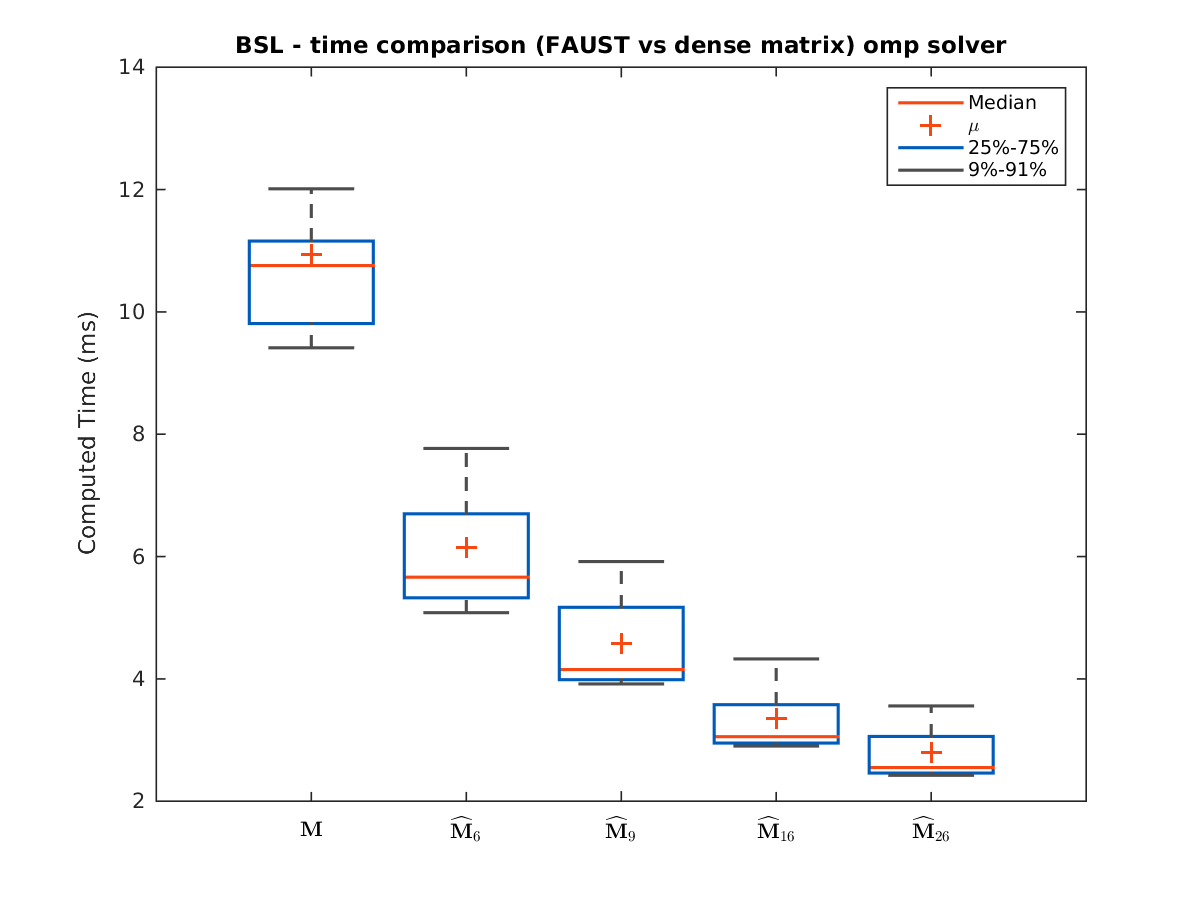
\includegraphics[scale=0.7]{images/BSL.png}
\end{figure}



%\section{Examples}\label{sec:example}

%\section{Other functions}\label{sec:other}

\bibliographystyle{plain}
\bibliography{paperbiblio}


\end{document}



